\documentclass[]{extarticle}
\usepackage[utf8]{inputenc}
\usepackage[letterpaper, margin=0.9in]{geometry}\usepackage{lipsum}
\usepackage{amsmath}
\usepackage{tikz}
\usepackage{amsfonts}
\usepackage{verbatim}
\usepackage{pdfpages}
\usepackage{cancel}
\usepackage{pdfpages}
\usepackage{float}
\usepackage{hyperref}
\usepackage{graphicx}
\usepackage{pgfplots}
\usepackage{subcaption}
\title{Project Work Plan}
\usetikzlibrary{positioning, arrows.meta}
\date{}



\usepackage{titlesec}

\setcounter{secnumdepth}{4}

\titleformat{\paragraph}
{\normalfont\normalsize\bfseries}{\theparagraph}{1em}{}
\titlespacing*{\paragraph}
{0pt}{3.25ex plus 1ex minus .2ex}{1.5ex plus .2ex}


\begin{document}

\begin{center}
    
\includegraphics[scale=0.8]{TAU.png}\\
    \vspace{1cm} % Adjust the length as needed
    
    \Large Project Work Plan\\
    \vspace{1cm} % Adjust the length as needed
    
    \large 2896\\
    \vspace{0.5cm} % Adjust the length as needed
    
    \large Designing Oscillator for an Antenna at \(\sim\)3.5 GHz\\
    \vspace{1cm} % Adjust the length as needed
    
\end{center}

\large {Students}:\\

Name: Nir Finch Cohen \ \ \ \ \ ID: 230336612\\

Name: Mazz Shaikh \ \ \ \ \ \ \ \ \ \  ID: 932056724\\

\vspace{1cm} % Adjust the length as needed

\large Project carried out at: Tel Aviv University\\
\vspace{1cm} % Adjust the length as needed

\large For the project instructor:\\
\vspace{0.3cm} % Adjust the length as needed

I approve the submission of the following report

\vspace{1cm} % Adjust the length as needed
\begin{flushright}
    \(\begin{matrix}
    \text{Signature:} &  \\ \\
    \text{Name:} & \text{Edoh Shaulov} \\
\end{matrix}\)
\end{flushright}

\newpage

\tableofcontents

\newpage

\section{Abstract}
\begin{comment}
The project abstract is a summary of the work in the project (≤ 2 pages).
This part should include explanations on the project subject, its field, where the technologies of the project are used, and an overview of the project implementation plan. This part should also include a block diagram of the project’s implementation. The block diagram should enable an engineer who does not read your entire work, understand your project content.
\end{comment}

%\subsection{Introduction to Project}

% Project Subject

In the ever-evolving landscape of wireless communications, the demand for efficient and reliable antennas operating at high frequencies has become paramount. This project delves into the implementation of an oscillator tailored for an antenna system at approximately 3.5 GHz. The oscillator is to be used in the transmitter antenna using a matching network. The significance of this endeavor lies in its potential to advance the performance of communication systems, catering to the ever-evolving landscape of modern connectivity. \\

% Project Field

The project delves into the field of Radio Frequency(RF) engineering, Microwave engineering and Analog Integrated Circuits. The intricacies of designing RF systems, especially those operating at high frequencies like 3.5 GHz, demand a meticulous understanding of circuit theory, analog circuits and frequency response, electromagnetic principles, and communication systems. \\


%\subsection{Potential uses}
% Uses of the technology

Oscillators are used in a diverse range of fields owing to their fundamental role in generating stable and precise periodic waveforms. The 3.5 GHz high-frequency oscillator to be developed as a part of this project finds profound uses in 5G networks and satellite communication. High-frequency oscillators are also used in radar systems for navigation, RFID tags in smartcards, and Magnetic Resonance Imaging (MRI). \\

In essence, the technologies harnessed in this project contribute not only to the advancement of 3.5 GHz antenna systems but also have far-reaching implications across industries, influencing the efficiency, precision, and reliability of diverse technological applications. \\

%\subsection{Project Plan}
The project unfolds systematically, with each phase carefully crafted to ensure the successful realization of a high-performance 3.5 GHz oscillator. The implementation plan encompasses the following key stages:

\begin{enumerate}
    \item Building an oscillator model \\
    The first step in the project starts by dealing with the 3.5 GHz oscillator. The model for the oscillator has to be tested using a Spice simulation.
    \item Component Selection \\
    This step involves choosing the right transistor (NPN BJT/ NMOS) and then finding an available transistor that works in the interested frequency interval. A spice model has to be made for the chosen transistor and simulated using Cadence Virtuoso for S-parameters.
    \item Antenna and it's matching \\
    The given oscillator design must have a matching network with the antenna we design. A matching network serves the crucial purpose of optimizing the transfer of power between two different components or systems that may have mismatched impedances. The primary use of a matching network is to ensure efficient power transfer and minimize signal reflections, particularly in the context of RF (Radio Frequency) and microwave systems.
    \item PCB Layout \\
    Create a compact and well-optimized printed circuit board (PCB) layout, taking into account RF design principles to minimize parasitic elements and signal loss.
    \item Testing \\
    The chip is tested with a pre-built receiver to check the integrity of the design.
    
\end{enumerate}


%\subsection{Block Diagram}

The project implements the Transmitter block shown in (Fig \ref{fig:block-diagram})

\begin{figure}[!h]
    \centering
    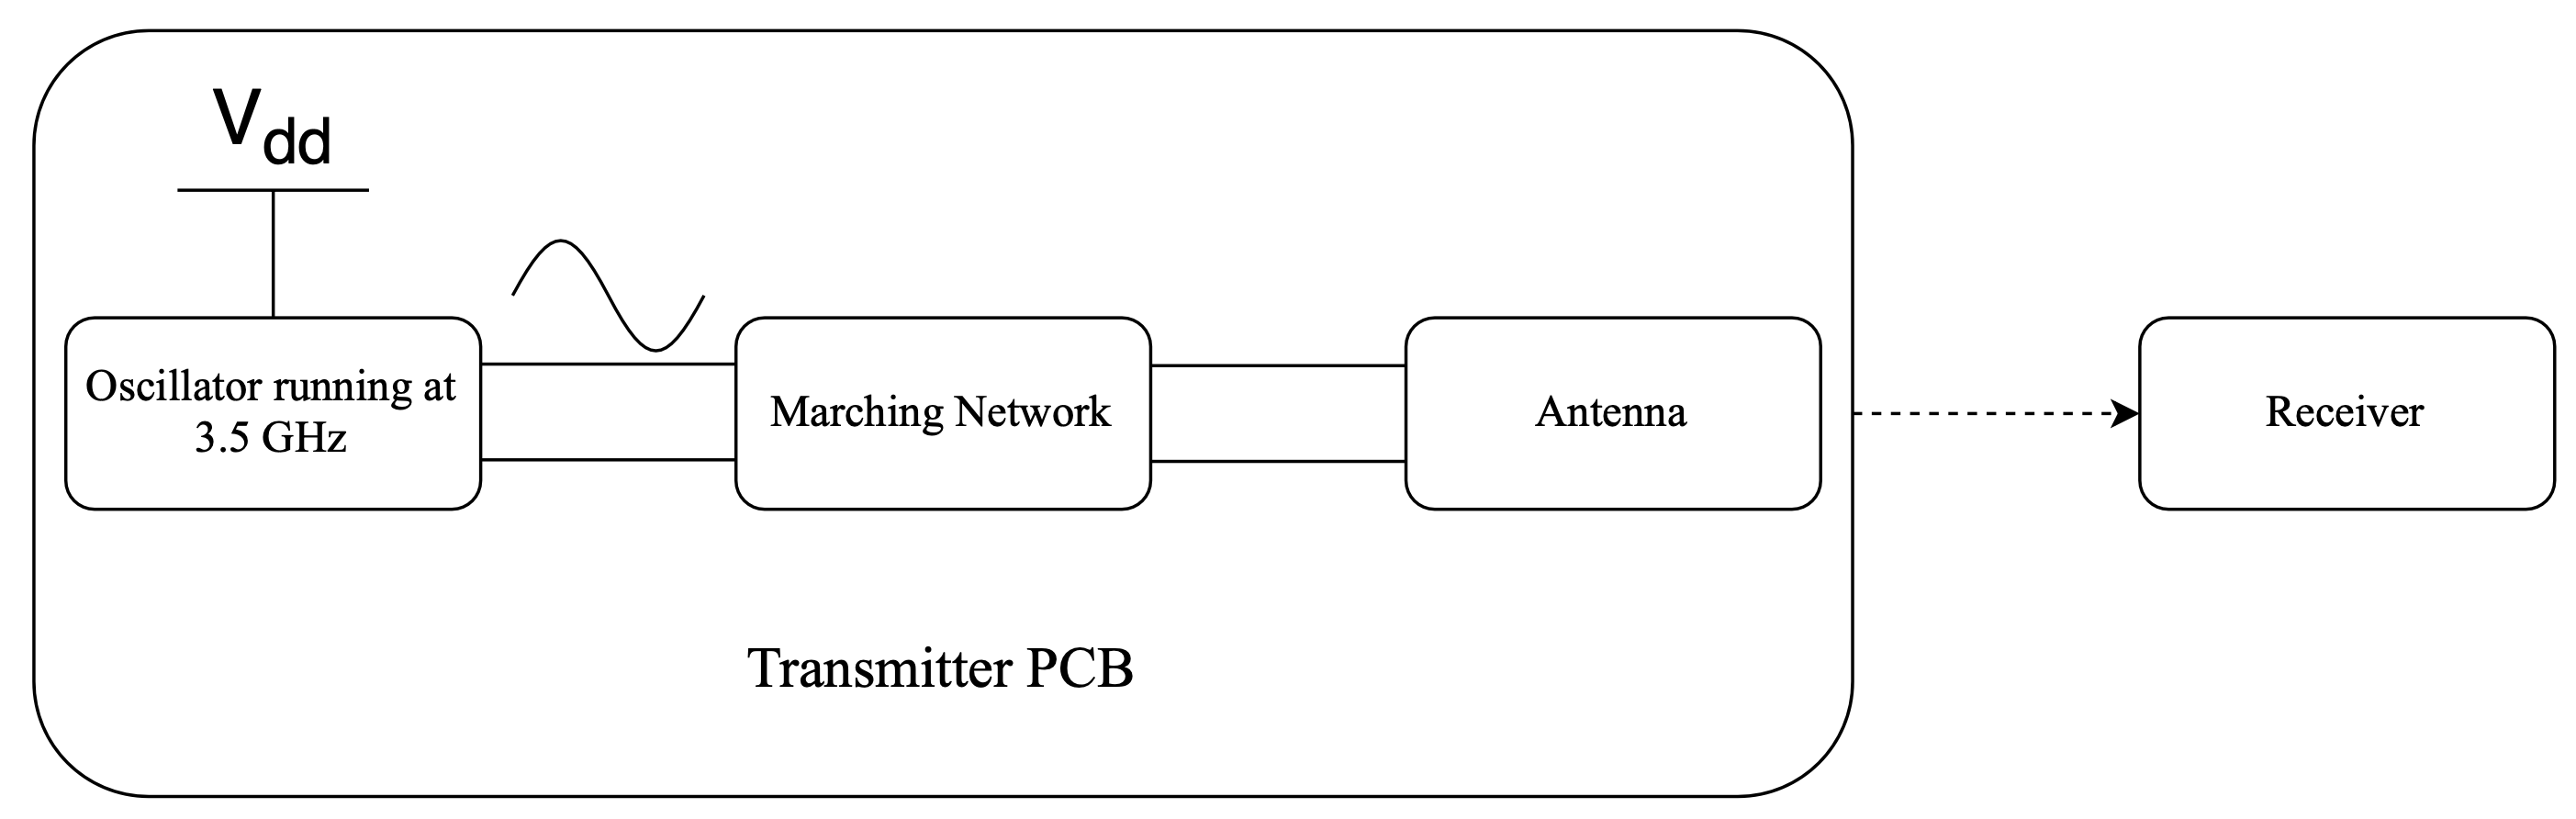
\includegraphics[width=0.8\linewidth]{block_diagram.png}
    \caption{Block Diagram for project}
    \label{fig:block-diagram}
\end{figure}

\newpage
\section{Motivation}
\begin{comment}
The motivation for the existence of this project (≤ 1page).
This part should include the scientific and engineering reasoning for this project, its importance and contribution, and in comparison to existing alternatives. (include at least 2 alternatives). This part should not include personal motivation for the project.
\end{comment}

At the core of this project lies a needed scientific challenge – the demand for precise and stable oscillations at the 3.5 GHz frequency. This frequency band has emerged in modern wireless communication systems, playing a pivotal role in 5G networks, satellite communication, and various other applications.\\

From an engineering perspective, the project is motivated by the pressing need to enhance the efficiency and reliability of antenna systems operating at 3.5 GHz. The oscillator, as the fundamental component dictating the frequency of the transmitted signal, directly influences the overall performance of the communication system. The design and implementation of a bespoke oscillator for this frequency band involve considerations of frequency stability, phase noise, and power efficiency.\\

Current solutions for high-frequency use single-ended oscillators(Fig \ref{fig:collpits}), using MOS or BJTs. However, single-ended Colpitts has some issues as then tend to exhibit higher phase noise compared to differential oscillators. Phase noise is a measure of the randomness of an oscillator's output, and it can degrade signal quality in applications where precise timing is critical. They are also susceptible to common-mode noise, which can interfere with the desired signal. To tackle the problems with single-ended oscillators, differential versions of collpits oscillators have been proposed(Fig \ref{fig:collpits-bjt-diff})~\cite{article}. \\ 

When operating at high frequencies, such as in the case of a high-frequency transmitter, the use of an off-the-shelf voltage-controlled oscillator (VCO) may fall short of meeting the stringent precision and frequency requirements demanded by the application. The design of a high-precision high-frequency transmitter necessitates a level of customization that generic VCOs may not afford. Thus, we build upon the two implementations stated above to have a more reliable system.

\begin{comment}
However, Bipolar Junction Transistors (BJTs) are often preferred for high-frequency oscillators when stability is a primary concern due to their superior performance characteristics in this domain. BJTs exhibit excellent high-frequency response, making them well-suited for applications where the oscillator needs to operate at elevated frequencies. Additionally, BJTs generally provide better thermal stability compared to other transistor types, ensuring that variations in temperature do not significantly impact the oscillator's performance. The inherent characteristics of BJTs, including low phase noise and high-frequency gain, contribute to stable and reliable oscillations in high-frequency applications, making them a favorable choice when stringent stability requirements are paramount. \\
\end{comment}

\newpage
\section{Statement of Work}

\begin{comment}
This section should elaborate on the work of the students in the project (≤ 2page). 
This section should start by elaborating on the theoretical background required for this project and the main sources for it. Next, continue by including a detailed description of the project requirements and the steps and methods required for this project including all steps required for all deliverables through the project and by its end (including any simulations, alternatives examinations, study, design, etc.). You should also include the mathematical/scientific/engineering/algorithmic theory required for this project. Indicate the tools, environment, and hardware required for every part of the project.
\end{comment}

\subsection{Theoretical Background}

\subsubsection{S-Parameters}


S-parameters, also known as scattering parameters, are a set of complex numbers that describe the linear relationships between waves entering and exiting a network of interconnected components. They are widely used in radio frequency (RF) and microwave engineering to characterize the performance of electronic circuits, antennas, and other devices.~\cite{Pozar:882338} \\

S-parameters are defined in terms of the incident, reflected, and transmitted waves at each port of the network. The incident wave is the wave entering the network, the reflected wave is the wave reflected back from the network, and the transmitted wave is the wave that passes through the network. The S-parameter matrix relates the phasors of the incident, reflected, and transmitted waves at each port.

\begin{equation}
    S = \begin{bmatrix}
        S_{11}&S_{12}&S_{13}&\dots&S_{1n}\\
        S_{21}&S_{22}&S_{23}&\dots&S_{2n}\\
        \vdots&&&\ddots&\\
        S_{m1}&S_{m2}&S_{m3}&\dots&S_{mn}\\
    \end{bmatrix}
    \label{eq: S-params}
\end{equation}
\\ 

S-parameters are typically measured using vector network analyzers (VNAs). A VNA applies a small signal to one port of the network and measures the complex reflection and transmission coefficients at all ports. The measured S-parameters can then be used to characterize the network's performance. S-parameters play a crucial role for analysis of operating frequency and matching in the project. \\


The S-parameters of a network have several physical interpretations. The magnitude of S11, for example, represents the reflection coefficient at port 1. A value of 1 indicates perfect reflection, while a value of 0 indicates no reflection. The magnitude of S21 represents the forward transmission coefficient, which is the ratio of the phasor of the transmitted wave at port 2 to the phasor of the incident wave at port 1. A value of 0 indicates no transmission, while a value of 1 indicates perfect transmission.


\subsubsection{Collpits Oscillators}

The Colpitts oscillator is a type of electronic oscillator that generates a sinusoidal waveform. It is a simple and versatile oscillator that can be used over a wide range of frequencies. The circuit consists of an inductor and two capacitors in parallel, which form a resonant tank circuit. The feedback for the active device is taken from a voltage divider made of the two capacitors. The oscillator is typically based on a bipolar junction transistor (BJT) or an operational amplifier (op-amp). It is also a very stable oscillator, which means that the frequency of the output waveform does not change much over time. This makes the Collpits oscillator a good choice for applications where frequency stability is important, such as radio transmitters and receivers. \\

\begin{figure}[!h]
    \centering
    \begin{subfigure}{0.45\textwidth}
        \centering
        
\includegraphics[width=0.35\textwidth]{collpits-oscilltor.png}
        \caption{Single-Ended Collpits Oscillator}
        \label{fig:collpits}
    \end{subfigure}
    \hspace{1cm} % Adjust the horizontal space between subfigures
    \begin{subfigure}{0.45\textwidth}
        \centering
        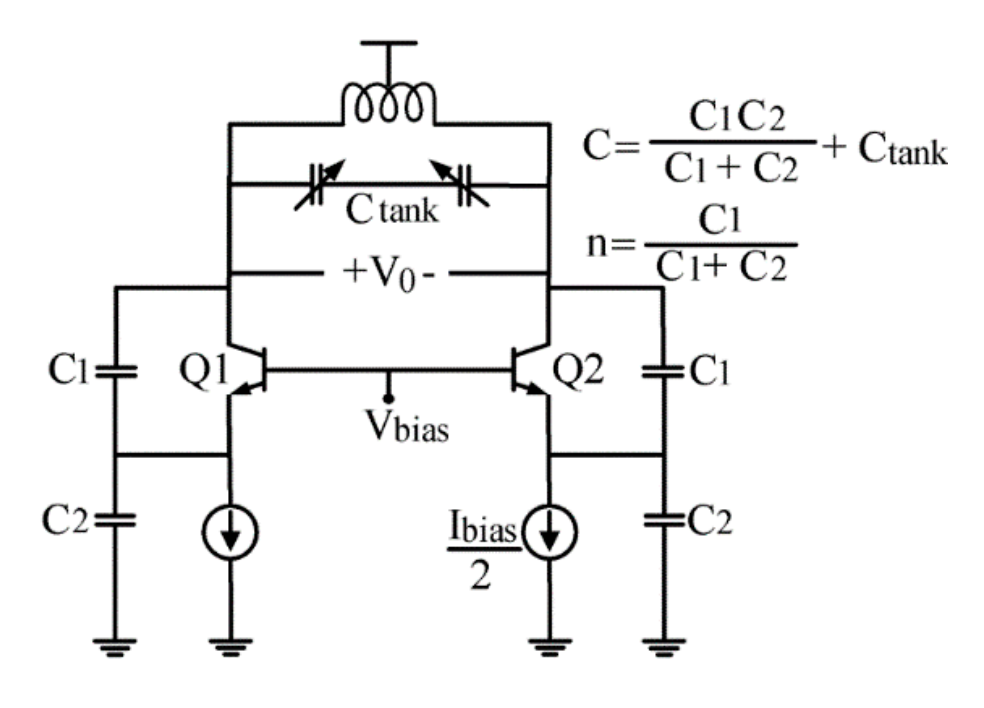
\includegraphics[width=\textwidth]{Collpits-BJT-Diff.png}
        \caption{Differential Collpits Oscillator using BJT}
        \label{fig:collpits-bjt-diff}
    \end{subfigure}
    \caption{Collpits Oscillators}
    \label{fig:combined}
\end{figure} 

\begin{figure}[!h]
    \centering
    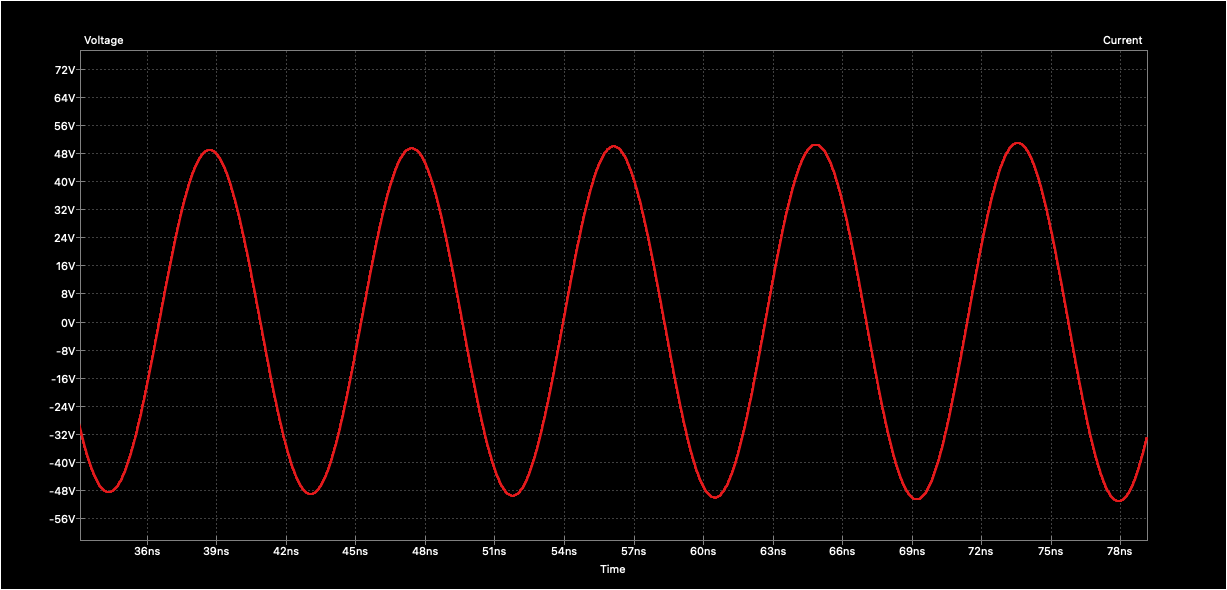
\includegraphics[width = 0.8\textwidth]{simulation.png}
    \caption{Differential Collpits Oscillator Simulation for Ideal NPN in \hyperref[https://ngspice.sourceforge.io]{NgSpice}}
    \label{fig:collpits-diff-sim}
\end{figure}

Here is a simplified explanation of how a Collpits oscillator works:~\cite{Razavi2001}

\begin{enumerate}
    \item The inductor and two capacitors form a resonant tank circuit. This circuit has a natural frequency at which it oscillates.
    \item The feedback amplifier amplifies the alternating current (AC) signal from the tank circuit.
    \item The feedback signal is fed back into the tank circuit, and the process repeats. This creates a positive feedback loop that sustains the oscillation.
\end{enumerate}

The frequency of the Colpitts oscillator can be controlled by changing the values of the inductor and capacitors in the tank circuit. The frequency of oscillation is given by 

\begin{equation}
    f_0 = \frac{1}{2\pi\displaystyle{\sqrt{L\frac{C_1C_2}{C_1+C_2}}}}
    \label{eg: collpits-freq-formula}
\end{equation}

\begin{comment}
To have oscillations, we must confide with Vendelin criteria
\begin{equation}
    k = \frac{1-|S_{11}|^2-|S_{22}|^2+|S_{11}S_{22}-S_{12}S_{21}|^2}{2|S_{12}||S_{21}|} < 1
\end{equation}
\end{comment}


However, single-ended Collpits has some issues as follows
\begin{enumerate}
    \item Higher phase noise: Single-ended Colpitts oscillators tend to exhibit higher phase noise compared to differential oscillators. Phase noise is a measure of the randomness of an oscillator's output, and it can degrade signal quality in applications where precise timing is critical.
    \item Lower common-mode rejection: Single-ended Colpitts oscillators are susceptible to common-mode noise, which can interfere with the desired signal.
\end{enumerate}


To address the limitations of single-ended Collpits oscillators, differential Collpits oscillators were developed using an extension of Collpits~\cite{article1} and other configurations~\cite{phdthesis}. These oscillators employ two active devices connected in a balanced configuration, resulting in improved performance(Fig \ref{fig:collpits-bjt-diff}). The two active devices generate a differential output signal, which is used to drive the resonant tank circuit and sustain the oscillation.



\subsubsection{Antenna and Matching Network}

 We design the antenna and match it to the oscillator using a matching network(Fig \ref{fig:block-diagram}). Matching networks, also known as impedance-matching circuits, are networks of passive components, such as inductors, capacitors, and transformers, that are used to match the impedance of a load to the impedance of a source. Impedance matching is an essential technique in RF engineering, as it can significantly improve the performance of RF systems. In RF systems, the impedance of the load and the impedance of the source must be matched to achieve maximum power transfer. If the impedances are not matched, there will be reflections of the signal, which will reduce the power transfer and lead to signal distortion. \\

The most straightforward matching-network topology is called the L network. This refers to eight different L-shaped circuits(Fig \ref{fig:matching-networks}) composed of two capacitors, two inductors, or one capacitor and one inductor. The exact method for matching will be developed in the later phases of the project. 

\begin{figure}[!h]
    \centering
    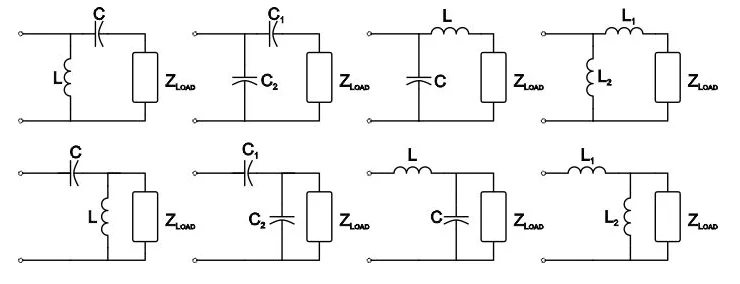
\includegraphics[width = 0.8\textwidth]{matching_networks.png}
    \caption{L-section Matching Networks}
    \label{fig:matching-networks}
\end{figure}
\subsection{Project Requirements}

The project requirements are as follows
\begin{enumerate}
    \item The circuit will support an input range of 5-20[V]
    \item The circuit will support frequencies up to 3.5[GHz]
    \item The oscillating frequency must not differ by more than 100[MHz] from the required target frequency
    \item The oscillator should function for a long time without decaying pulse
    
\end{enumerate}


\subsection{Required environment and tools}
\begin{enumerate}
    \item Designing Oscillator using Cadence PSpice:
    \begin{itemize}
        \item Utilize Cadence PSpice for the design and simulation of the oscillator circuit.
        \item Implement and validate the oscillator circuit in PSpice, considering real-world transistor characteristics.
        \item Analyze simulation results to ensure stability, frequency accuracy, and harmonic content meet project requirements.
    \end{itemize}

    \item Testing S-Parameters and Matching using Cadence Virtuoso:
    \begin{itemize}
        \item Employ Cadence Virtuoso for testing S-parameters and optimizing the matching network.
        \item Simulate the matching network design to achieve a \(50[\Omega]\) impedance match for the antenna.
        \item Analyze S-parameters, including return loss and insertion loss, to validate the effectiveness of the matching network.
    \end{itemize}

    \item Testing the Antenna using EMF Simulation using CTS/MATLAB:
    \begin{itemize}
        \item Use CTS (Circuit Telecommunication Simulation) and MATLAB for electromagnetic field (EMF) simulation of the antenna system.
        \item Simulate the antenna's radiation characteristics, efficiency, and impedance matching in realistic environmental conditions.
        \item Analyze simulation results to ensure the antenna meets specified requirements and integrates seamlessly with the overall transmitter system.
    \end{itemize}
\end{enumerate}

\newpage
\section{Project Deliverables}
\begin{comment}
You should outline the project deliverables (<1 page): Please outline and describe the project deliverables and take into account that some of the deliverables must be submitted before the progress presentation submission, in the end of the first semester.
A deliverable should be more than a theoretical abstract and should contain at least some simulation results.
Please include in your deliverables list: 
1.	A description of the system requirements: at least 3 quantized requirements the project must achieve.
2.	Specify all simulations, designs, developing and testing of algorithms, prototypes, etc.
3.	Specify which methods and tests will be performed on the project outcomes and describe the testing environment.
\end{comment}

To achieve the project objectives, the following detailed deliverables have been outlined:

\begin{enumerate}
    \item {Working Spice Model of Chosen Transistor:}
    \begin{itemize}
        \item Develop and validate a detailed Spice model for the selected transistor.
        \item Conduct simulations to demonstrate the transistor's functionality and performance characteristics.
        \item Include results such as voltage-current characteristics, frequency response, and transient analysis.
    \end{itemize}

    \item {Oscillator Design and Simulation:}
    \begin{itemize}
        \item Design an oscillator circuit capable of generating the required frequency.
        \item Simulate the oscillator performance using both ideal and real transistor models.
        \item Present simulation results in time domain, FFT analysis, and S-parameters in Virtuoso.
        \item Include detailed analyses of stability, frequency accuracy, and harmonic content.
    \end{itemize}

    \item {Matching Network Design and S-Parameters Analysis:}
    \begin{itemize}
        \item Design a matching network to achieve a \(50[\Omega]\) impedance match for the antenna.
        \item Simulate the matching network and present S-parameters to validate the impedance matching.
    \end{itemize}

    \item {Antenna System Implementation:}
    \begin{itemize}
        \item Develop and simulate the antenna system to be integrated into the transmitter.
        \item Include simulation results demonstrating antenna efficiency, radiation patterns, and impedance characteristics.
    \end{itemize}

    \item {Transmitter Simulation and PCB Layout:}
    \begin{itemize}
        \item Simulate the entire transmitter system, incorporating the oscillator, matching network, and antenna.
        \item Utilize an EMF simulator to assess electromagnetic compatibility and ensure proper functioning.
        \item Create a detailed PCB layout considering optimal component placement for signal integrity.
        \item Conduct simulations to validate the PCB layout's impact on signal quality and interference.
    \end{itemize}

    \item {PCB Fabrication and System Testing:}
    \begin{itemize}
        \item Fabricate the PCB according to the finalized layout.
        \item Conduct testing using a pre-built receiver to validate the overall system performance.
        \item Include test results such as signal strength, frequency accuracy, and reliability.
        \item Document any issues encountered during testing and propose potential solutions.
    \end{itemize}
\end{enumerate}

\newpage
\section{Project Schedule}
\begin{comment}
A table with the main milestones (13-16 milestones). Please include a brief description of a milestone. The highlighted milestones are mandatory. (<= 1page)
\end{comment}


\begin{tabular}{|c|p{5cm}|p{9cm}|c|}
    \hline
    & Milestones & Description & Date \\
    \hline
    1 & Paper review & Conduct a thorough review of relevant literature and research papers to establish a foundation for the project. & 15/1 \\
    \hline
    2 & Choosing an oscillator model to build upon & Evaluate and select a suitable oscillator model as the basis for further development. Consider factors such as stability and frequency range. & 21/1 \\
    \hline
    3 & Building Ideal Single-Ended Oscillator Model and Simulating for S-parameters & Construct an ideal single-ended oscillator model and perform simulations to analyze S-parameters, ensuring initial functionality. & 21/2 \\
    \hline
    4 & Building the Differential counterpart and Simulating for S-parameters & Extend the oscillator model to a differential configuration, simulating and analyzing S-parameters for enhanced performance. & 28/2 \\
    \hline
    5 & Choosing transistor, building its spice model and using it in place of ideal one & Identify a suitable transistor, develop its Spice model, and integrate it into the oscillator model, replacing the idealized component. & 14/3 \\
    \hline
    6 & \textbf{Progress Presentation Submission} &  &  \\
    \hline
    7 & Reserach on Antenna matching  & Reading papers related to antenna matching for design inspirations & 21/3 \\
    \hline
    8 & Building a matching assuming antenna to be \(50[\Omega]\) & Design a matching network under the assumption of a \(50[\Omega]\) antenna impedance. Simulate and optimize for effective impedance matching. & 14/4 \\
    \hline
    9 & Using Antenna with required impedance & Develop an antenna system with the specified impedance characteristics, considering radiation patterns and efficiency. & 14/5 \\
    \hline
    10 & \textbf{Poster Submission and finishing the work} &  &  \\
    \hline
    11 & PCB layout & Design the printed circuit board (PCB) layout, considering optimal component placement& 1/6 \\
    \hline
    12 & PCB fabrication& Fabricating the design & 1/8 \\
    \hline
    13 & Testing Transmitter & Conduct comprehensive testing of the assembled transmitter system to validate its functionality and performance. & 7/8 \\
    \hline
    14 & \textbf{Final deliverables submission} & & \\
    \hline
\end{tabular}



% -------------------------- references --------------------------
\newpage
\bibliographystyle{plain}
\bibliography{references.bib}

\end{document}
